\documentclass[12pt, letterpaper]{article}
\usepackage[titletoc,title]{appendix}
\usepackage{booktabs}
\usepackage[usenames,dvipsnames,svgnames,table]{xcolor}
\definecolor{dark-red}{rgb}{0.75,0.10,0.10}
\usepackage[margin=1in]{geometry}
\usepackage[linkcolor=dark-red,
            colorlinks=true,
            urlcolor=blue,
            citecolor={dark-red},
            pdftitle={Covered}]{hyperref}
\usepackage{graphicx}
\usepackage{amsfonts,amssymb,amsbsy}
\usepackage{natbib}
\setcitestyle{round,semicolon,aysep={},yysep={;}}
\usepackage{setspace}
\usepackage{chngcntr}
\usepackage[hang, font=small,skip=0pt, labelfont={bf}]{caption}
\setlength{\parindent}{3em}

% Generated by scripts/make_paper_assets.py -- do not edit.
% Every inline number in the manuscript comes from here, so the paper
% cannot drift out of step with the data.
\newcommand{\ClipDirectHi}{74}
\newcommand{\ClipDirectLo}{55}
\newcommand{\CodabilityCorr}{0.82}
\newcommand{\CommentatorShare}{23.8}
\newcommand{\DistinctRoles}{530,124}
\newcommand{\ExecLegRatio}{11}
\newcommand{\ExecShare}{14.8}
\newcommand{\GuestTurns}{6,764,038}
\newcommand{\LegShare}{1.4}
\newcommand{\LiveDirectHi}{44}
\newcommand{\LiveDirectLo}{27}
\newcommand{\MeasuredShare}{71.6}
\newcommand{\MediaShare}{13.5}
\newcommand{\ModeGapMedian}{27}
\newcommand{\ModeGapMin}{18}
\newcommand{\ModeGapYears}{25}
\newcommand{\ModeYears}{25}
\newcommand{\NMI}{0.65}
\newcommand{\PrincipalShare}{25.4}
\newcommand{\PrivateShare}{9.5}
\newcommand{\UnknownShare}{25.5}


\title{Covered: Who Speaks on Cable News, and What Do They Bring?\\\vspace{10mm}}
\author{Gaurav Sood\thanks{Gaurav can be reached at:
  \href{mailto:gsood07@gmail.com}{\texttt{gsood07@gmail.com}}.}}

\begin{document}
\maketitle
\doublespacing

Journalism's central convention is attribution. Rather than assert, reporters
cite---and the citation is meant to do epistemic work, transferring warrant from
a source to a claim \citep{tuchman1972}. Who gets cited is therefore not merely
a question about access. It is a question about what kind of evidence the news
rests on.

The sociology of news has long counted sources by their institutional home, and
found officials dominant \citep{sigal1973, gans1979, bennett1990}. But
institutional home and evidentiary standing are different things, and counting
only the first conflates them. A prosecutor trying the case being covered and a
former prosecutor booked to opine about it occupy the same sector and stand in
completely different relations to the facts. The first was there; the second is
guessing, expertly. Existing schemes---including recent computational ones that
assign each source a single label \citep{morlan2025, spangher2024}---cannot
express that difference.

We measure sources on two crossed axes. \emph{Sector} is the institutional home:
government, judiciary, business, academy, media, private individual, and so on.
\emph{Epistemic role} is why the source is cited: as the principal whose conduct
is the news, as a spokesperson for an institution, as a participant in the
events, as an eyewitness, from personal experience, as a credentialed expert, or
as a commentator with no privileged access. Normalized mutual information
between the axes is $\NMI$, so about a third of the epistemic axis is
information the sector does not carry.

That third is not spread evenly, and Table~\ref{tab:crossing} is candid about
where it lives. In several sectors the epistemic role is close to determined:
academics are cited as experts, other outlets' journalists as commentators,
performers as principals, and the second axis buys nothing. The crossing pays
where role descriptions vary within a sector---courts and law, private
individuals, party operatives, the executive branch---and those are exactly the
places where the distinction matters most. It is also where the paper's claims
are concentrated.

The corpus is \GuestTurns{} external-guest speaker turns from CNN transcripts,
2000--2025, with \DistinctRoles{} distinct role descriptions. US cable
transcripts label speakers as \texttt{NAME, ROLE:}, so the affiliation is
supplied in the text rather than inferred, which is what makes classical
measurement viable at this scale. Supporting Information \ref{si_taxonomy}
describes the coding.

\section*{What a network plays is not what it books}

The clearest result concerns a distinction available only in broadcast. A
transcript separates people the network \emph{books} to appear live from people
whose recorded words it \emph{plays}, and these are different editorial acts.
They are also epistemically different. Figure~\ref{fig:mode} shows the share of
turns from sources with direct access to the events---principals, participants,
eyewitnesses, and people speaking from personal experience.

\begin{figure}[htbp]
  \centering
  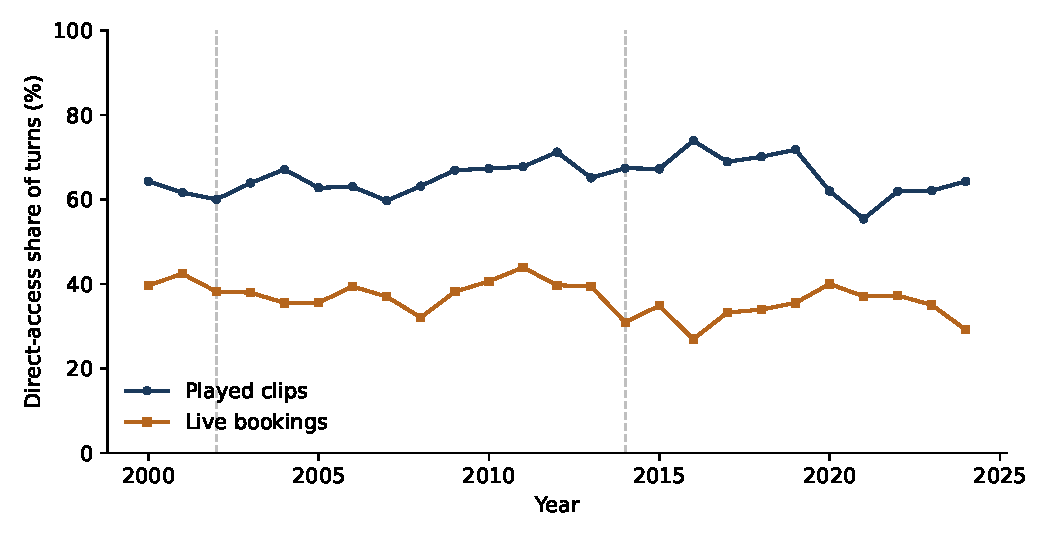
\includegraphics[width=\textwidth]{../figs/proximity_by_mode.pdf}
  \caption{Share of guest turns from sources with direct access to the events
    reported, by whether the turn is a live booking or a played clip. Dashed
    lines mark transcript-format boundaries. The gap holds in every year of the
    corpus.}
  \label{fig:mode}
\end{figure}

Played clips run \ClipDirectLo--\ClipDirectHi\% direct access; live bookings
\LiveDirectLo--\LiveDirectHi\%. Clips exceed bookings in \ModeGapYears{} of
\ModeYears{} years, by a median of \ModeGapMedian{} percentage points and never
by fewer than \ModeGapMin{}. Clips carry evidence; bookings carry talk. Because
this is a within-year comparison, it is unaffected by the measurement drift
discussed below.

The asymmetry is easy to rationalize after the fact---a clip is played
\emph{because} someone said something consequential, while a booking fills an
hour---but it has an uncomfortable implication. The share of airtime given to
live panels rather than played material is, in effect, a choice about how much
of the broadcast rests on evidence.

\section*{The executive crowds out everyone else in government}

\begin{table}[htbp]
\centering\footnotesize\setlength{\tabcolsep}{3pt}
\caption{Institutional sector by epistemic role, CNN guest turns, 2000--2025. Row percentages; \% turns is each sector's share of all guest turns. \emph{Unres.} is reported rather than dropped: it is the share the role text does not settle. $H$ is the normalised entropy of each row: sectors near zero are ones the sector alone already determines, where the second axis adds nothing.}
\label{tab:crossing}
\begin{tabular}{lrrrrrrrrrrr}
\hline\hline
Sector & Prin. & Spok. & Part. & Eyew. & Exp'ce & Expert & Comm. & Pop. & Unres. & \% turns & $H$ \\
\hline
Government, executive & 69.5 & 10.3 & 0.2 & 0.0 & 0.0 & 0.4 & 19.7 & 0.0 & 0.0 & 14.8 & 0.38 \\
Government, legislative & 78.5 & 0.2 & 0.1 & 0.0 & 1.5 & 0.0 & 19.7 & 0.0 & 0.0 & 1.4 & 0.27 \\
Government, subnational & 65.7 & 0.5 & 0.2 & 0.0 & 0.6 & 0.0 & 33.0 & 0.1 & 0.0 & 0.9 & 0.33 \\
Judicial and legal & 7.0 & 0.1 & 16.2 & 0.0 & 0.0 & 5.3 & 71.3 & 0.0 & 0.0 & 6.1 & 0.40 \\
Law enforcement & 2.8 & 69.7 & 5.1 & 0.0 & 0.0 & 22.2 & 0.1 & 0.0 & 0.0 & 2.5 & 0.39 \\
Military & 5.0 & 7.8 & 56.1 & 0.0 & 0.4 & 30.3 & 0.3 & 0.1 & 0.0 & 1.6 & 0.49 \\
Party and campaign & 37.7 & 4.7 & 5.7 & 0.0 & 0.0 & 0.0 & 51.9 & 0.0 & 0.0 & 3.3 & 0.46 \\
Business & 94.8 & 0.5 & 0.0 & 0.0 & 0.0 & 0.1 & 4.6 & 0.0 & 0.0 & 4.4 & 0.10 \\
Academic & 0.1 & 0.1 & 0.0 & 0.0 & 0.0 & 99.7 & 0.1 & 0.0 & 0.0 & 3.3 & 0.01 \\
Think tank & 5.6 & 0.0 & 0.0 & 0.7 & 0.0 & 93.3 & 0.4 & 0.0 & 0.0 & 0.5 & 0.13 \\
Nonprofit and advocacy & 2.7 & 93.4 & 0.0 & 0.2 & 0.7 & 0.7 & 2.3 & 0.0 & 0.0 & 0.9 & 0.15 \\
Labor union & 25.7 & 64.8 & 0.2 & 0.0 & 0.1 & 0.2 & 9.0 & 0.0 & 0.0 & 0.0 & 0.40 \\
Religious & 0.6 & 91.3 & 0.5 & 0.0 & 1.4 & 0.7 & 5.5 & 0.1 & 0.0 & 0.3 & 0.18 \\
Media (other outlets) & 0.1 & 0.1 & 0.0 & 0.2 & 0.0 & 0.1 & 99.5 & 0.0 & 0.0 & 13.5 & 0.02 \\
Professional & 0.2 & 0.0 & 0.1 & 0.0 & 0.3 & 98.7 & 0.7 & 0.0 & 0.0 & 3.9 & 0.04 \\
Entertainment and sport & 96.4 & 0.1 & 0.0 & 0.0 & 0.1 & 0.1 & 3.4 & 0.0 & 0.0 & 7.4 & 0.08 \\
Private individual & 0.0 & 0.1 & 7.7 & 12.7 & 71.8 & 0.0 & 0.4 & 7.4 & 0.0 & 9.5 & 0.42 \\
Unknown & 0.6 & 2.5 & 0.1 & 0.0 & 0.1 & 0.0 & 0.8 & 0.1 & 95.8 & 25.5 & 0.10 \\
\hline\hline
\end{tabular}
\end{table}


Table~\ref{tab:crossing} gives the joint distribution. Executive-branch sources
are \ExecShare\% of guest turns; legislative sources are \LegShare\%, a ratio of
about \ExecLegRatio{} to one. Cable news covering national politics is
overwhelmingly covering the executive.

This is a supply-side counterpart to a demand-side finding. Asked which
political leaders come to mind, survey respondents name prominent
ones---disproportionately presidents and presidential candidates---rather than
ideologically extreme ones, and that paper closed by conjecturing that the bias
lies less in who is covered than in how \citep{sood_recall}. On the first half
of the conjecture, the supply side is at least consistent with the demand side:
the executive branch is what television shows.

\section*{Ordinary people, and why they are hard to count}

Private individuals are \PrivateShare\% of guest turns: relatives, neighbours,
witnesses, survivors, defendants, refugees, volunteers. This is Gans's
category of ``unknowns,'' people who reach the news through deviance or
misfortune rather than position \citep{gans1979}.

That figure is a floor, and the reason is itself a finding. How reliably a role
description can be classified depends on how often it recurs, because recurring
descriptions are standardized job titles and one-off descriptions are not. Among
role strings we \emph{can} classify, composition shifts sharply with rarity
(Table~\ref{tab:rarity} in \ref{si_coverage}): private individuals and people
speaking from personal experience are far more common among rare strings, and
commentators far less. Uncodable strings are rarer than codable ones. So the
residue we cannot classify is disproportionately ordinary people speaking from
direct experience, and \PrivateShare\% understates them.

The mechanism deserves stating plainly. Television labels its pundits in
reusable ways and the people things happen to in bespoke ways---\textsc{former
fbi director} recurs; \textsc{haleigh's baby-sitter} does not. Any instrument
keyed on role descriptions will therefore find the powerful easier to count than
the powerless, and will understate the latter unless it says so. Ours currently
leaves \UnknownShare\% of turns with no sector, and reports that share rather
than distributing it.

\section*{What we cannot say}

We set out to measure whether the evidentiary basis of cable news has changed
over twenty-five years, and we cannot answer it with these data. The direct
access share is flat across the period, and what moves instead is the split
between experts and commentators, which tracks the news cycle rather than time:
in 2020 commentary fell and expert testimony rose; in 2024 the reverse. But the
more basic problem is that classifiability itself trends upward over the period
($r = \CodabilityCorr$ with year), because CNN moved from idiosyncratic interview
television toward standardized political panels. Worst-case bounds on the direct
share are then roughly two and a half times wider than the between-year
variation they would have to resolve. Program fixed effects absorb rather more
than half the variance in classifiability but under half its trend.

We report this because the alternative---presenting a series whose movement is
indistinguishable from the instrument's improvement---would be worse than
reporting nothing.

\clearpage
% apsr.bst is not in this machine's TeX tree; apalike is the closest style that
% ships with a base install. Swap to apsr where it is available (as in
% ../extreme_recall) -- both are natbib author-year, so no citation changes.
\bibliographystyle{apalike}
\bibliography{covered}

\clearpage
\appendix
\renewcommand{\thesection}{SI \arabic{section}}
\setcounter{table}{0}\renewcommand\thetable{\thesection.\arabic{table}}
\counterwithin{figure}{section}

\begin{center}
\Large{Supporting Information}
\end{center}

\section{The taxonomy}\label{si_taxonomy}

Each speaker turn is parsed from the \texttt{NAME, ROLE:} label. A role clause
is written only at a speaker's first mention; later turns are bare surnames, so
roles are propagated within a transcript from a roster, and whether a role was
read locally or inherited is recorded.

Two independent lexicons map keywords to sector and to epistemic role. Matching
is longest-keyword-wins on whole words, so row order in the lexicon files is
irrelevant and a new keyword cannot shadow an existing one. Because the axes are
matched separately, they compose: \textsc{pentagon spokesman} resolves to
military $\times$ spokesperson without either file enumerating the pair.

Three attributes are lifted out of the role clause before matching, because they
describe delivery or affiliation rather than the kind of source: how the speaker
reached air (\emph{voice-over}, \emph{via telephone}, \emph{through
translator}), a party tag, and standing (\emph{current}, \emph{former},
\emph{candidate}). Standing then modifies the epistemic role: leaving a post
ends the standing that made someone a principal, a spokesperson or a
participant, so a former officeholder is coded as a commentator. Where authority
is a credential rather than a post, whether the source is an expert or a
commentator depends on the segment topic, and those cells are flagged rather
than guessed.

When no keyword matches, three fallbacks apply in order: a typographic
convention by which an outlet name alone denotes a visiting journalist; an
honorific in the speaker's name (US legislators are written \textsc{sen.\ john
mccain, (r) arizona}, putting the office in the name and only party and state in
the role); and a frozen per-string dictionary for descriptions no rule
generalizes to. Every label records which route produced it.

\section{Coverage and what is missing}\label{si_coverage}

\begin{table}[htbp]
\centering\small
\caption{Epistemic composition of codable role strings, by how often the string recurs. Quintiles of string frequency; percentages within quintile. Categories over-represented among rare strings are the ones the uncoded residual is mostly made of, and are therefore under-counted in Table~\ref{tab:crossing}.}
\label{tab:rarity}
\begin{tabular}{lrrr}
\hline\hline
Epistemic role & Rarest \% & Commonest \% & Gap (pp) \\
\hline
Comm. & 16.5 & 33.0 & -16.5 \\
Prin. & 34.1 & 34.6 & -0.5 \\
Pop. & 0.8 & 1.0 & -0.2 \\
Expert & 11.5 & 11.5 & -0.1 \\
Eyew. & 3.1 & 1.5 & +1.6 \\
Part. & 6.1 & 3.8 & +2.2 \\
Spok. & 10.2 & 6.1 & +4.2 \\
Exp'ce & 17.6 & 8.5 & +9.1 \\
\hline\hline
\end{tabular}
\end{table}


Table~\ref{tab:rarity} reports epistemic composition of classifiable role
strings by quintile of how often the string recurs. Read the gap column as the
sign of the bias in Table~\ref{tab:crossing}: categories over-represented among
rare strings are what the unclassified residue is mostly made of, and are
therefore undercounted.

Epistemic roles are read from the text for \MeasuredShare\% of turns; the
remainder fall back on what the sector implies, and are marked as such
throughout so that any table can be recomputed without them.

One consequence deserves stating. Some keywords fix both axes at once---a
professor is academic and an expert---so for sectors whose role vocabulary is
homogeneous, the epistemic label is partly an artifact of how the lexicon is
built rather than an independent reading of the text. The $H$ column in
Table~\ref{tab:crossing} makes those rows visible, and the aggregate mutual
information should be read as an average over sectors that differ a great deal
in how much the second axis is doing.

\section{Validation}\label{si_validation}

\textbf{[VALIDATION PENDING]} A stratified probability sample of speaker turns,
double-coded, will supply: inter-coder agreement per axis; a confusion matrix
per axis rather than a headline accuracy; and recall by sector and by epistemic
role separately, since differential recall---not average accuracy---is what
biases composition estimates \citep{asr2021}. An external check is available at
no cost: a sister corpus of MSNBC transcripts ships a human-authored guest list
for every transcript, sharing no code with this pipeline.

\end{document}
